\documentclass{classrep}
\usepackage[utf8]{inputenc}
\frenchspacing

\usepackage{graphicx}
\usepackage[usenames,dvipsnames]{color}
\usepackage[hidelinks]{hyperref}
\usepackage{float}
\usepackage{setspace}
\usepackage{amsmath, amssymb, mathtools}
\usepackage{rotating}

\usepackage{booktabs}
\usepackage{graphicx}
\usepackage{pdflscape}
\usepackage{lscape}

\setlength{\abovecaptionskip}{-10pt}

\studycycle{Informatyka stosowana, studia dzienne, II st.}
\coursesemester{II}
\coursename{Analiza danych złożonych}
\courseyear{2020/2021}

\courseteacher{dr hab. inż. Agnieszka Duraj}
\coursegroup{poniedziałek, 11:45}

\author{%
  \studentinfo{Paweł Galewicz}{234053}\\
  \studentinfo{Karol Podlewski}{234106}%
}

\title{Etap 3: Badanie podobieństwa oraz przynależności zbiorów tekstowych}

\begin{document}
\maketitle

\setstretch{1.5}

\tableofcontents
\setstretch{1.25}
\newpage


\section{Cel}

Zadanie polegało na analizie zbioru danych pod kątem podobieństwa atrybutów tekstowych oraz przynależności atrybutów numerycznych do określonych etykiet.

\section{Implementacja}

Program został stworzony w języku Python w wersji 3.8.6. Wyniki zostały zapisane w skoroszycie Excel za pomocą biblioteki \textit{openpyxl}. Do wygenerowania wykresów przynależności wykorzystano bibliotekę \textit{matplotlib}. Podobieństwo atrybutów tekstowych sprawdzano z wykorzystaniem wzoru Niewiadomskiego. Dla atrybutów numerycznych określono etykiety na podstawie charakterystyki zbioru i nadano im trapezowe funkcje przynależności.

\section{Opis teoretyczny}

W sprawozdaniu wykorzystano następujące zagadnienia.


\subsection{Zbiory rozmyte}

Niech X będzie przestrzenią o skończonej liczbie elementów, wówczas zbiorem
rozmytym A określonym na przestrzeni X nazywamy zbiór par w postaci

\begin{center}
    $A = \{< x, \mu_A(x) >: x \in X\}, x \in X$
\end{center}

gdzie $\mu_A(x)$ jest funkcją przynależności wyrażoną jako

\begin{center}
    $\mu_A(x): X \rightarrow [0,1]$    
\end{center}

i określającą stopień przynależności elementu x do zbioru A.\\

Rozszerzeniem zbioru rozmytego jest przedziałowy zbiór rozmyty, dla którego definiowane są dwie funkcje przynależności - dolna i górna. Oznaczają one odpowiednio minimalny i maksymalny stopień przynależności elementu.

\begin{center}
    $A = \{< x, \underline{\mu_A(x)}, \overline{\mu_A(x)} >: x \in X\}, x \in X$
\end{center}

gdzie 

\begin{center}
    $\underline{\mu_A(x)}, \overline{\mu_A(x)}: X \rightarrow [0;1]$
\end{center}

oraz 

\begin{center}
    $0 \le \underline{\mu_A(x)} \le \overline{\mu_A(x)} \le 1$
\end{center}

\subsection{Podobieństwo tekstu}

Podobieństwo słów $s_1$ i $s_2$
zdefiniować można następującym wzorem:

\begin{figure}[H]
    \centering
    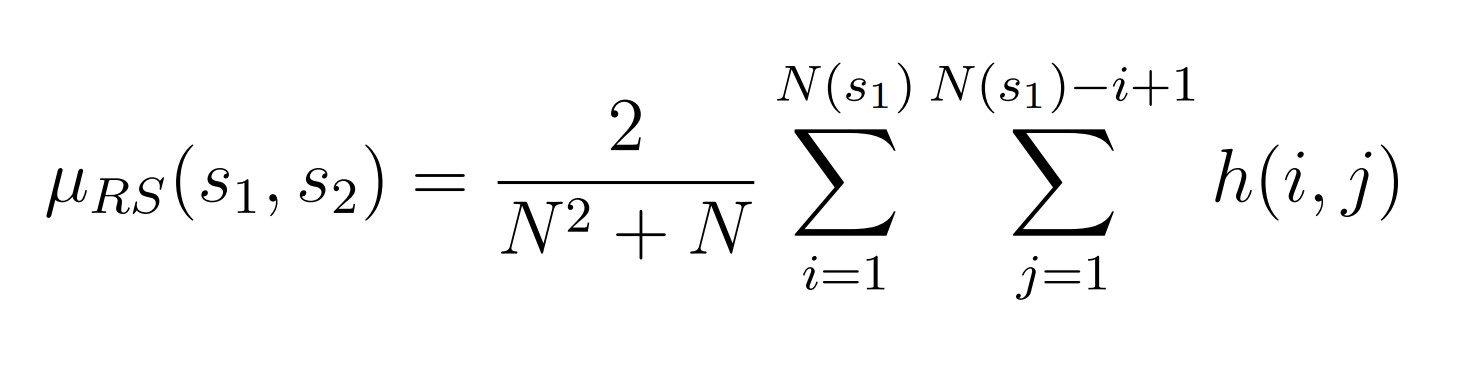
\includegraphics[width=0.55\textwidth]{resources/stage3/words.jpg}
\end{figure}

w którym ${N}$ definiowane jest jako maksymalna długość słów $s_1$ i $s_2$, zaś ${h(i, j)}$ przyjmuje wartość 1 gdy podciąg i-elementowy liter występujący w słowie $s_1$ i rozpoczynający się od
j-tego miejsca w słowie $s_1$ występuje co najmniej raz w słowie $s_2$, a 0, jeżeli podciąg i-elementowy liter występujący w słowie $s_1$ i rozpoczynający się od j-tego miejsca w słowie $s_1$ nie występuje w słowie $s_2$.

Korzystając z powyższego wzoru zdefiniować możemy funkcję podobieństwa zdań $z_1$ i $z_2$, wyrażoną następującym wzorem:

\begin{figure}[H]
    \centering
    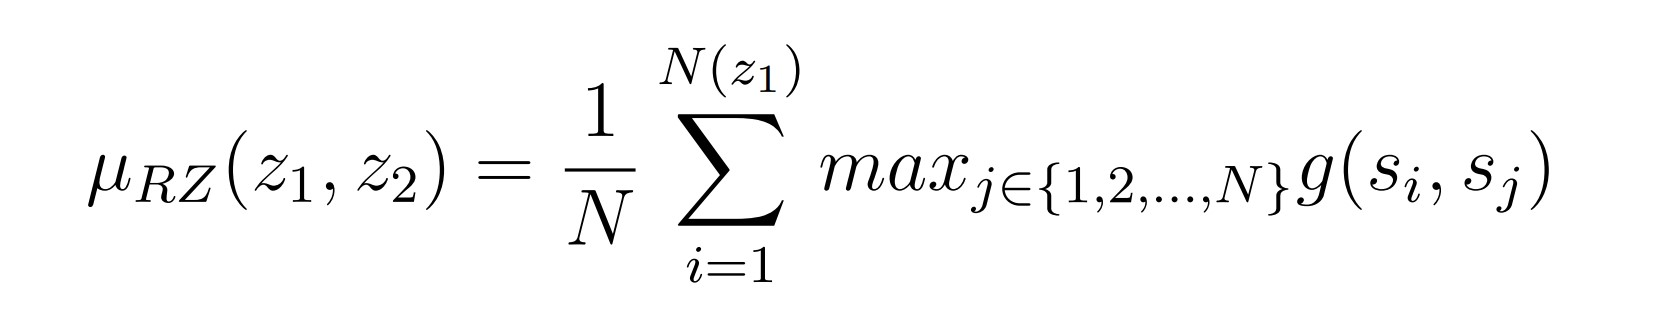
\includegraphics[width=0.6\textwidth]{resources/stage3/text.jpg}
\end{figure}

gdzie $N$ jest maksymalną liczbą słów $z_1$ i $z_2$, a $g(s_i, s_j)$ jest funkcją podobieństwa słów $s_i$ i $s_2$.

\subsection{Współczynnik R}

Współczynnik r atrybutów \textit{R, S} dla których etykiety zdefiniowane są odpowiednio $a_1, a_2, a_3$ i $b_1, b_2, b_3$  wyrażony jest wzorem:
\begin{center}
$r = \frac{ \sum\nolimits_{i=1}^{n} [ \mu_R (a_i) * \mu_S (b_i)]}{\sum\nolimits_{i=1}^{n} \mu_R (a_i)}$
\end{center}

\section{Zbiór danych}

Do zadania wykorzystano zbiór wpisów na portalu Tweeter - dalej zwanych \textit{tweetami} - dotyczących zmian klimatycznych. Zbiór pobrano z platformy Kaggle \cite{db}. Zbiór zawiera ok. 400 rekordów zawierających treść wpisu oraz metadane dotyczące jego oraz jego autora. Do analizy wybrano następujące atrybuty:

\begin{itemize}
    \item twitter\_name -- nazwa użytkownika z portalu Tweeter, autora tweeta
    \item text -- tekst tweeta
    \item followers -- liczba osób obserwujących autora tweeta
    \item likes -- liczba polubień tweeta
    \item polarity -- odbiór tweeta przez innych użytkowników prezentowana liczbą z przedziału [-1, 1], gdzie -1 oznacza negatywny odbiór, zaś 1 oznacza pozytywny odbiór
\end{itemize}

Na potrzeby wyznaczenia etykiet oraz wzorów przynależności dla liczbowych atrybutów: followers, likes, polarity wyznaczono statystyki zaprezentowane Tabeli \ref{stats}.

\begin{table}[H]
    \caption{Statystyki wybranych atrybutów numerycznych}
    \label{stats}
    \centering
    \begin{tabular}{|l|l|l|l|}
        \hline
              & followers & likes & polarity \\ \hline
        mean  & 11472.44  & 6.74  & 0.04     \\ \hline
        std   & 95007.77  & 46.87 & 0.14     \\ \hline
        min   & 0         & 0     & -0.5     \\ \hline
        25\%  & 132       & 0     & 0        \\ \hline
        50\%  & 1069      & 0     & 0        \\ \hline
        75\%  & 4191.25   & 2     & 0.12     \\ \hline
        max   & 1720089   & 88.0  & 0.6      \\ \hline
    \end{tabular}
\end{table}

\section{Badania}

W ramach analizy przeprowadzono następujące zadania.

\subsection{Porównanie tekstu tweetów}

Do analizy wykorzystano atrybut text. W ramach badania porównane zostały wszystkie tweety ze sobą i na podstawie wyników stworzono macierz, w której w kolumnami i rzędami są tweety, a na przecięciu wpisany jest wyliczony współczynnik podobieństwa tweetów. Wynikowa tabela znajduje się w arkuszu \textit{Tweets similarity}, a jej poglądową część prezentuje Tabela \ref{similarity}.

\begin{table}[H]
    \caption{Porównanie tekstu tweetów}
    \label{similarity}
    \centering
    \begin{tabular}{llllllll}
        \cline{1-6} \cline{8-8}
        \multicolumn{1}{|l|}{Similarity} &
          \multicolumn{1}{l|}{Tweet 1} &
          \multicolumn{1}{l|}{Tweet 2} &
          \multicolumn{1}{l|}{Tweet 3} &
          \multicolumn{1}{l|}{Tweet 4} &
          \multicolumn{1}{l|}{Tweet 5} &
          \multicolumn{1}{c|}{} &
          \multicolumn{1}{l|}{Tweet 396} \\ \cline{1-6} \cline{8-8} 
        \multicolumn{1}{|l|}{Tweet 1} &
          \multicolumn{1}{l|}{1} &
          \multicolumn{1}{l|}{0,342888} &
          \multicolumn{1}{l|}{0,299971} &
          \multicolumn{1}{l|}{0,251233} &
          \multicolumn{1}{l|}{0,226598} &
          \multicolumn{1}{l|}{} &
          \multicolumn{1}{l|}{0,381816} \\ \cline{1-6} \cline{8-8} 
        \multicolumn{1}{|l|}{Tweet 2} &
          \multicolumn{1}{l|}{0,209888} &
          \multicolumn{1}{l|}{1} &
          \multicolumn{1}{l|}{0,312124} &
          \multicolumn{1}{l|}{0,225024} &
          \multicolumn{1}{l|}{0,189221} &
          \multicolumn{1}{l|}{} &
          \multicolumn{1}{l|}{0,311165} \\ \cline{1-6} \cline{8-8} 
        \multicolumn{1}{|l|}{Tweet 3} &
          \multicolumn{1}{l|}{0,214364} &
          \multicolumn{1}{l|}{0,312775} &
          \multicolumn{1}{l|}{1} &
          \multicolumn{1}{l|}{0,402763} &
          \multicolumn{1}{l|}{0,346178} &
          \multicolumn{1}{c|}{...} &
          \multicolumn{1}{l|}{0,326685} \\ \cline{1-6} \cline{8-8} 
        \multicolumn{1}{|l|}{Tweet 4} &
          \multicolumn{1}{l|}{0,113415} &
          \multicolumn{1}{l|}{0,130878} &
          \multicolumn{1}{l|}{0,243279} &
          \multicolumn{1}{l|}{1} &
          \multicolumn{1}{l|}{0,468254} &
          \multicolumn{1}{l|}{} &
          \multicolumn{1}{l|}{0,157893} \\ \cline{1-6} \cline{8-8} 
        \multicolumn{1}{|l|}{Tweet 5} &
          \multicolumn{1}{l|}{0,12073} &
          \multicolumn{1}{l|}{0,122297} &
          \multicolumn{1}{l|}{0,212279} &
          \multicolumn{1}{l|}{0,490781} &
          \multicolumn{1}{l|}{1} &
          \multicolumn{1}{l|}{} &
          \multicolumn{1}{l|}{0,161802} \\ \cline{1-6} \cline{8-8} 
        \multicolumn{1}{c}{} &
           &
           &
          \multicolumn{1}{c}{...} &
           &
           &
           &
          \multicolumn{1}{c}{} \\ \cline{1-6} \cline{8-8} 
        \multicolumn{1}{|l|}{Tweet 396} &
          \multicolumn{1}{l|}{0,277615} &
          \multicolumn{1}{l|}{0,348182} &
          \multicolumn{1}{l|}{0,346694} &
          \multicolumn{1}{l|}{0,265106} &
          \multicolumn{1}{l|}{0,262948} &
          \multicolumn{1}{c|}{} &
          \multicolumn{1}{l|}{1} \\ \cline{1-6} \cline{8-8} 
    \end{tabular}
\end{table}

\subsection{Przynależność z wykorzystaniem zbiorów rozmytych}

Do badań przynależności wykorzystano atrybuty followers, likes, polarity. Każdemu z atrybutów nadano etykietę, do którego stworzono funkcję przynależności w następujący sposób:

\begin{itemize}
    \item Dla atrybutu followers etykietę "Tweet author is very popular", której funkcję przynależności prezentuje Rysunek \ref{very_popular}
    \item Dla atrybutu likes etykietę "Tweet has no likes", której funkcję przynależności prezentuje Rysunek \ref{not_liked}
    \item Dla atrybutu polarity etykietę "Tweet was neutrally received", której itemize przynależności prezentuje Rysunek \ref{neutrally_received}
\end{itemize}

\begin{figure}[H]
    \centering
    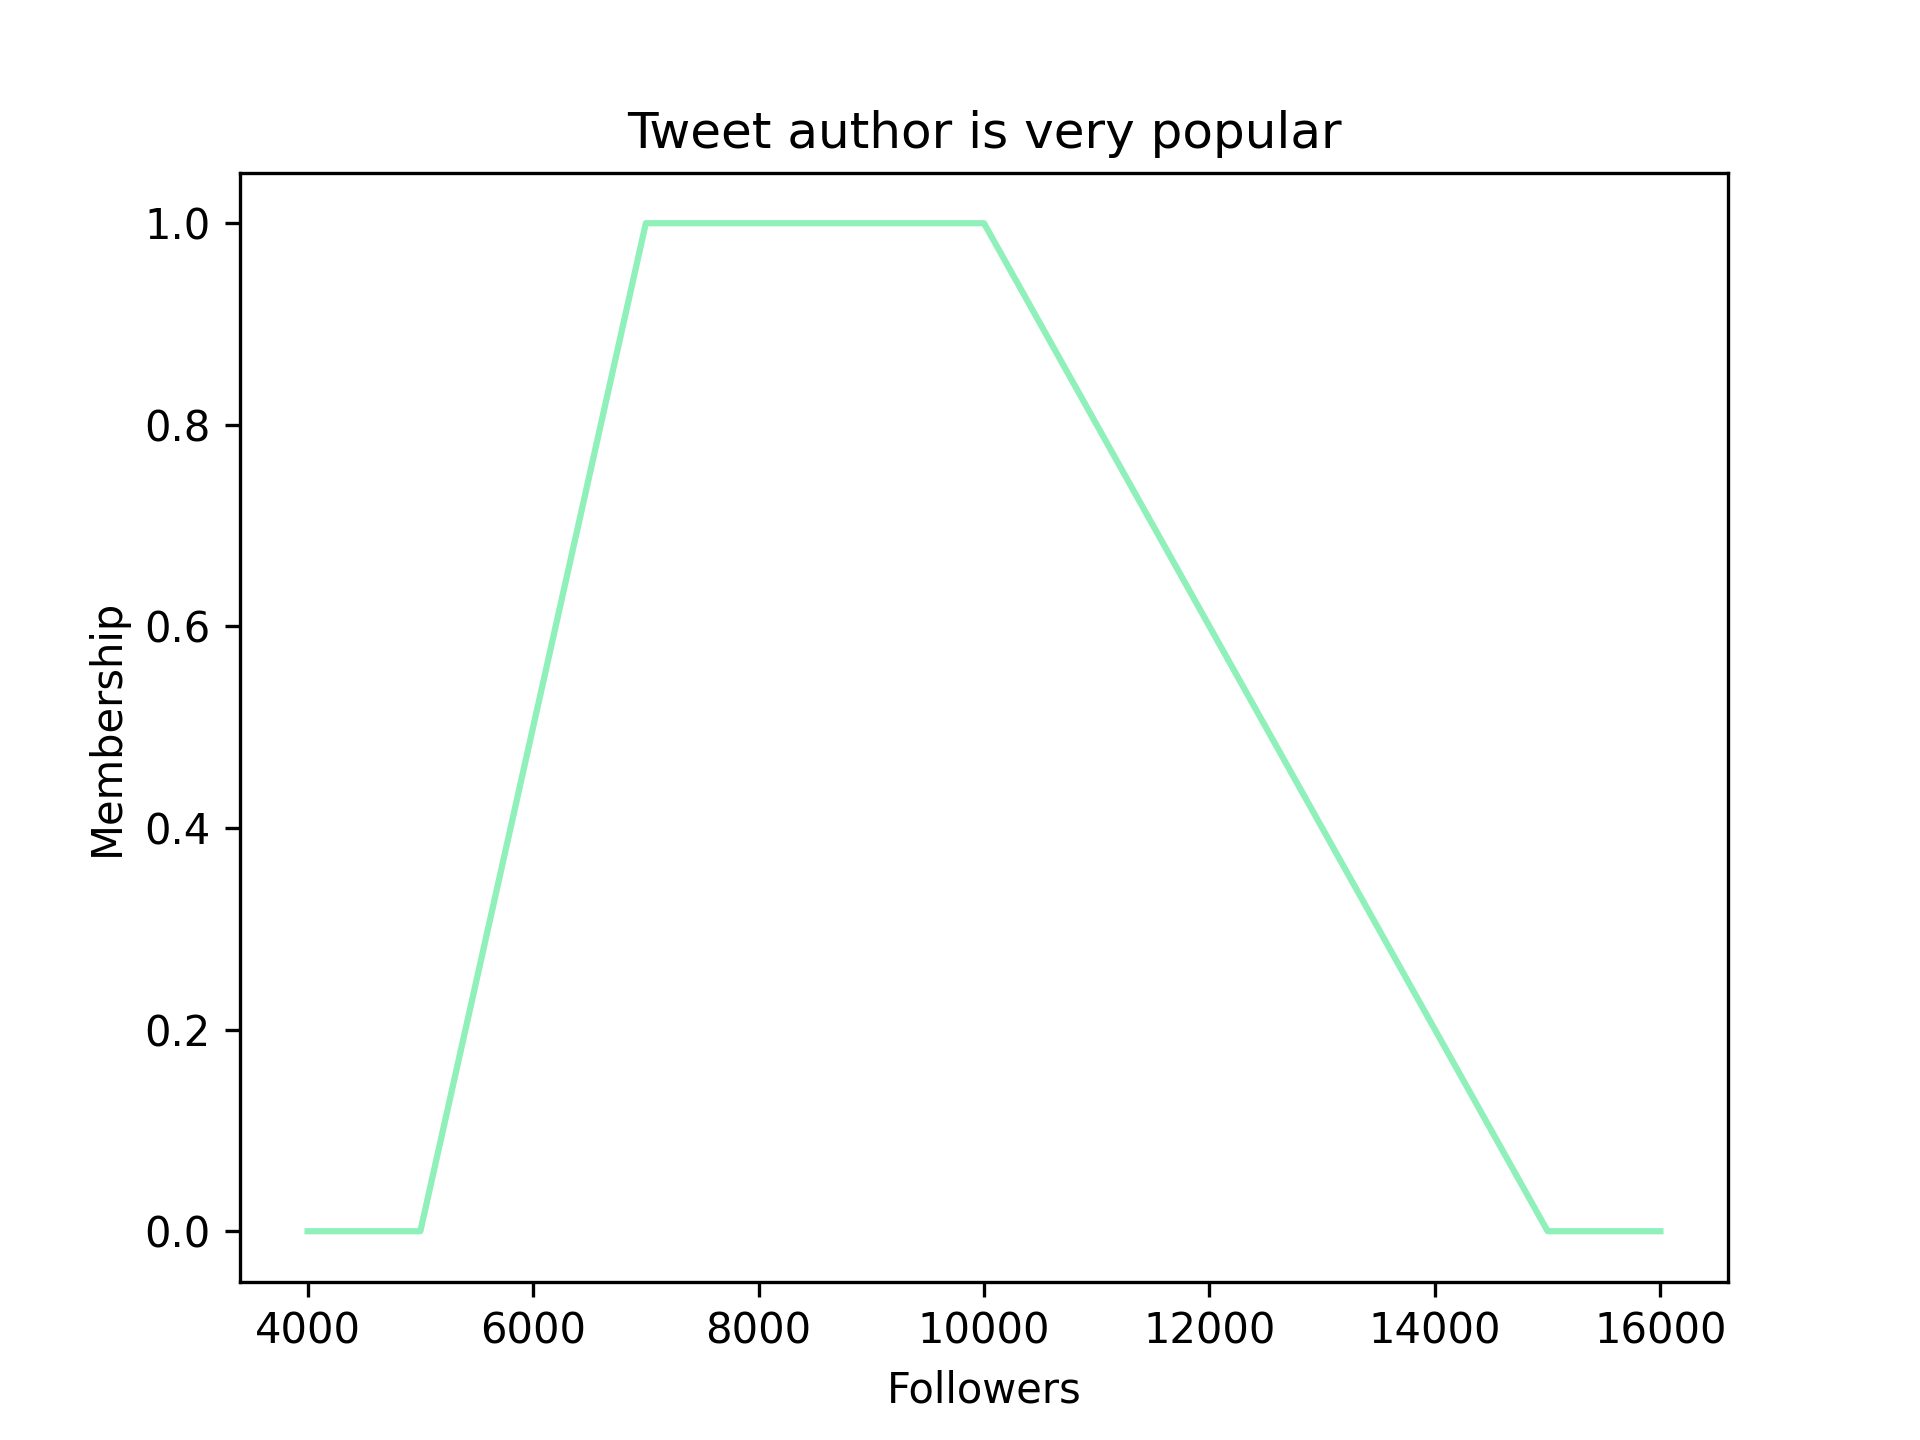
\includegraphics[width=1\textwidth]{resources/stage3/Tweet author is very popular.png}
    \caption{Funkcja przynależności dla atrybutu followers}
    \label{very_popular}
\end{figure}

\begin{figure}[H]
    \centering
    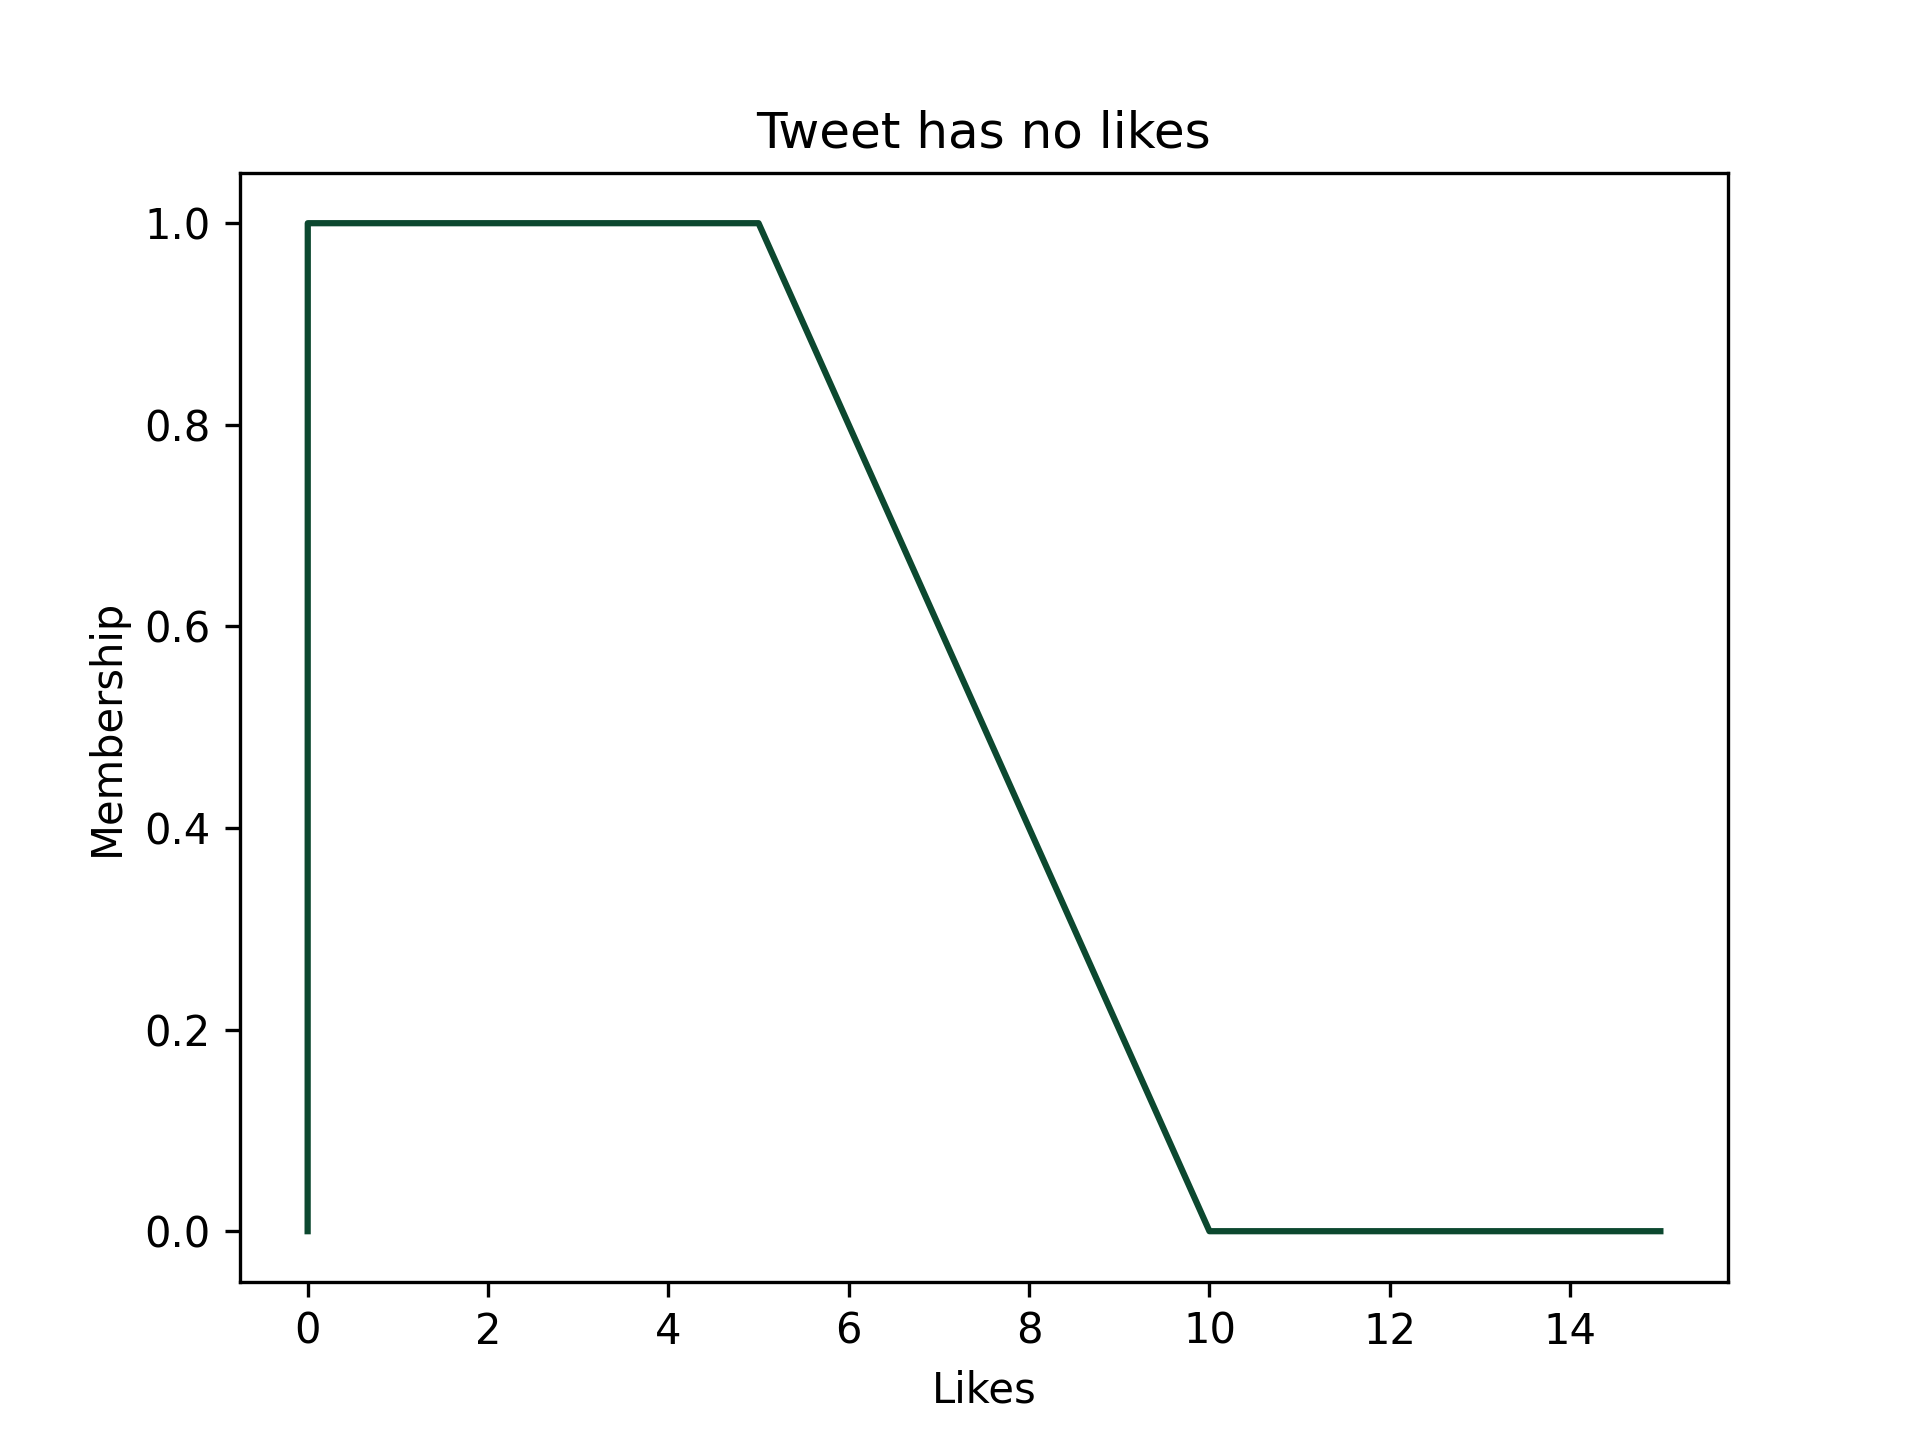
\includegraphics[width=1\textwidth]{resources/stage3/Tweet has no likes.png}
    \caption{Funkcja przynależności dla atrybutu likes}
    \label{not_liked}
\end{figure}

\begin{figure}[H]
    \centering
    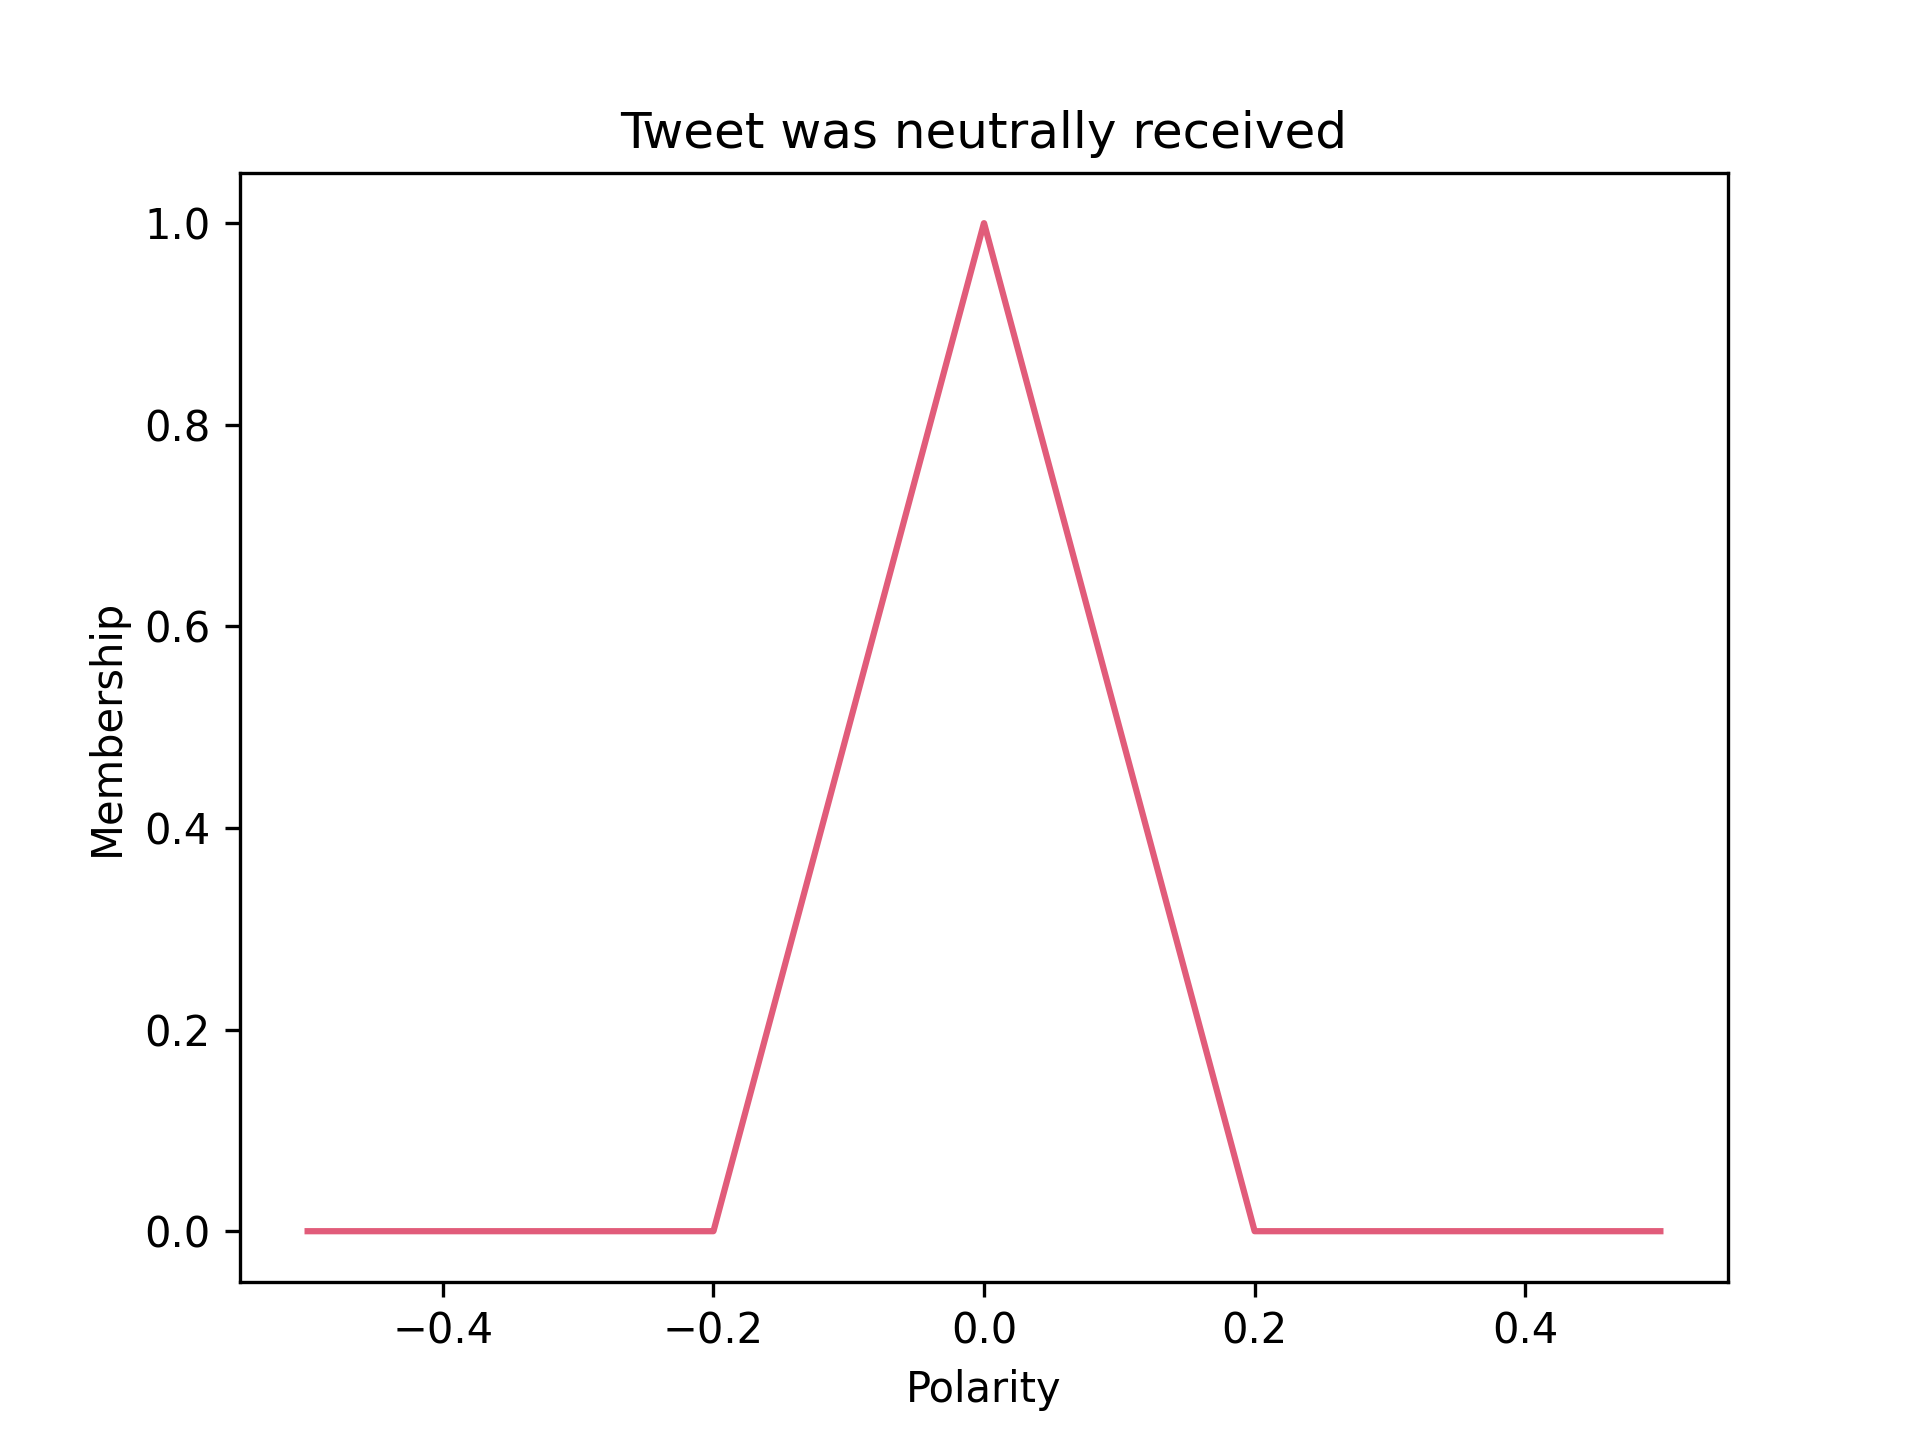
\includegraphics[width=1\textwidth]{resources/stage3/Tweet was neutrally received.png}
    \caption{Funkcja przynależności dla atrybutu polarity}
    \label{neutrally_received}
\end{figure}

Dla każdego tweeta wyliczono wartości przynależności funkcji i zapisano w arkuszu \textit{Fuzzy membership}, którego poglądową część zaprezentowano w Tabeli \ref{fuzzy}

\begin{table}[H]
    \caption{Wartości funkcji przynależności tweetów}
    \label{fuzzy}
    \centering
    \begin{tabular}{lllll}
        \hline
        \multicolumn{1}{|l|}{Author} &
          \multicolumn{1}{l|}{Tweet} &
          \multicolumn{1}{l|}{Tweet has no likes} &
          \multicolumn{1}{l|}{\begin{tabular}[c]{@{}l@{}}Tweet was \\ neutrally recieved\end{tabular}} &
          \multicolumn{1}{l|}{\begin{tabular}[c]{@{}l@{}}Tweet author\\ is very popular\end{tabular}} \\ \hline
        \multicolumn{1}{|l|}{ECOWARRIORSS}    & \multicolumn{1}{l|}{\{Treść\}} & \multicolumn{1}{l|}{0} & \multicolumn{1}{l|}{0,73} & \multicolumn{1}{l|}{0}    \\ \hline
        \multicolumn{1}{|l|}{ElsevierEnergy}  & \multicolumn{1}{l|}{\{Treść\}} & \multicolumn{1}{l|}{0} & \multicolumn{1}{l|}{0}    & \multicolumn{1}{l|}{0,80} \\ \hline
        \multicolumn{1}{|l|}{siwarr5}         & \multicolumn{1}{l|}{\{Treść\}} & \multicolumn{1}{l|}{1} & \multicolumn{1}{l|}{0}    & \multicolumn{1}{l|}{0}    \\ \hline
        \multicolumn{1}{|l|}{EDITORatWORK}    & \multicolumn{1}{l|}{\{Treść\}} & \multicolumn{1}{l|}{0} & \multicolumn{1}{l|}{1}    & \multicolumn{1}{l|}{0}    \\ \hline
        \multicolumn{1}{|l|}{EDITORatWORK}    & \multicolumn{1}{l|}{\{Treść\}} & \multicolumn{1}{l|}{1} & \multicolumn{1}{l|}{1}    & \multicolumn{1}{l|}{0}    \\ \hline
        \multicolumn{1}{|l|}{mapsofworld}     & \multicolumn{1}{l|}{\{Treść\}} & \multicolumn{1}{l|}{0} & \multicolumn{1}{l|}{0,39} & \multicolumn{1}{l|}{0,15} \\ \hline
        \multicolumn{1}{|l|}{EnvirHealthNews} & \multicolumn{1}{l|}{\{Treść\}} & \multicolumn{1}{l|}{1} & \multicolumn{1}{l|}{0}    & \multicolumn{1}{l|}{0,95} \\ \hline
                                              &                                & \multicolumn{1}{c}{}   & ...                       &                           \\ \hline
        \multicolumn{1}{|l|}{TheDailyClimate} & \multicolumn{1}{l|}{\{Treść\}} & \multicolumn{1}{l|}{0} & \multicolumn{1}{l|}{0,44} & \multicolumn{1}{l|}{0}    \\ \hline
    \end{tabular}
\end{table}

\subsection{Przynależność z wykorzystaniem przedziałowych zbiorów rozmytych}

Dla tych samych atrybutów nadano inne etykiety, dla których tym razem stworzono funkcje przynależności z wykorzystaniem przedziałowych zbiorów rozmytych. Etykiety prezentują się następująco:

\begin{itemize}
    \item Dla atrybutu followers etykietę "Tweet author is moderately popular", której funkcję przynależności pokazano na Rysuneku \ref{moderately_popular}
    \item Dla atrybutu likes etykietę "Tweet has a lot of likes", której funkcję przynależności pokazano na Rysuneku \ref{very_liked}
    \item Dla atrybutu polarity etykietę "Tweet was negatively received", której funkcję przynależności pokazano na Rysuneku \ref{negatively_received}
\end{itemize}

\begin{figure}[H]
    \centering
    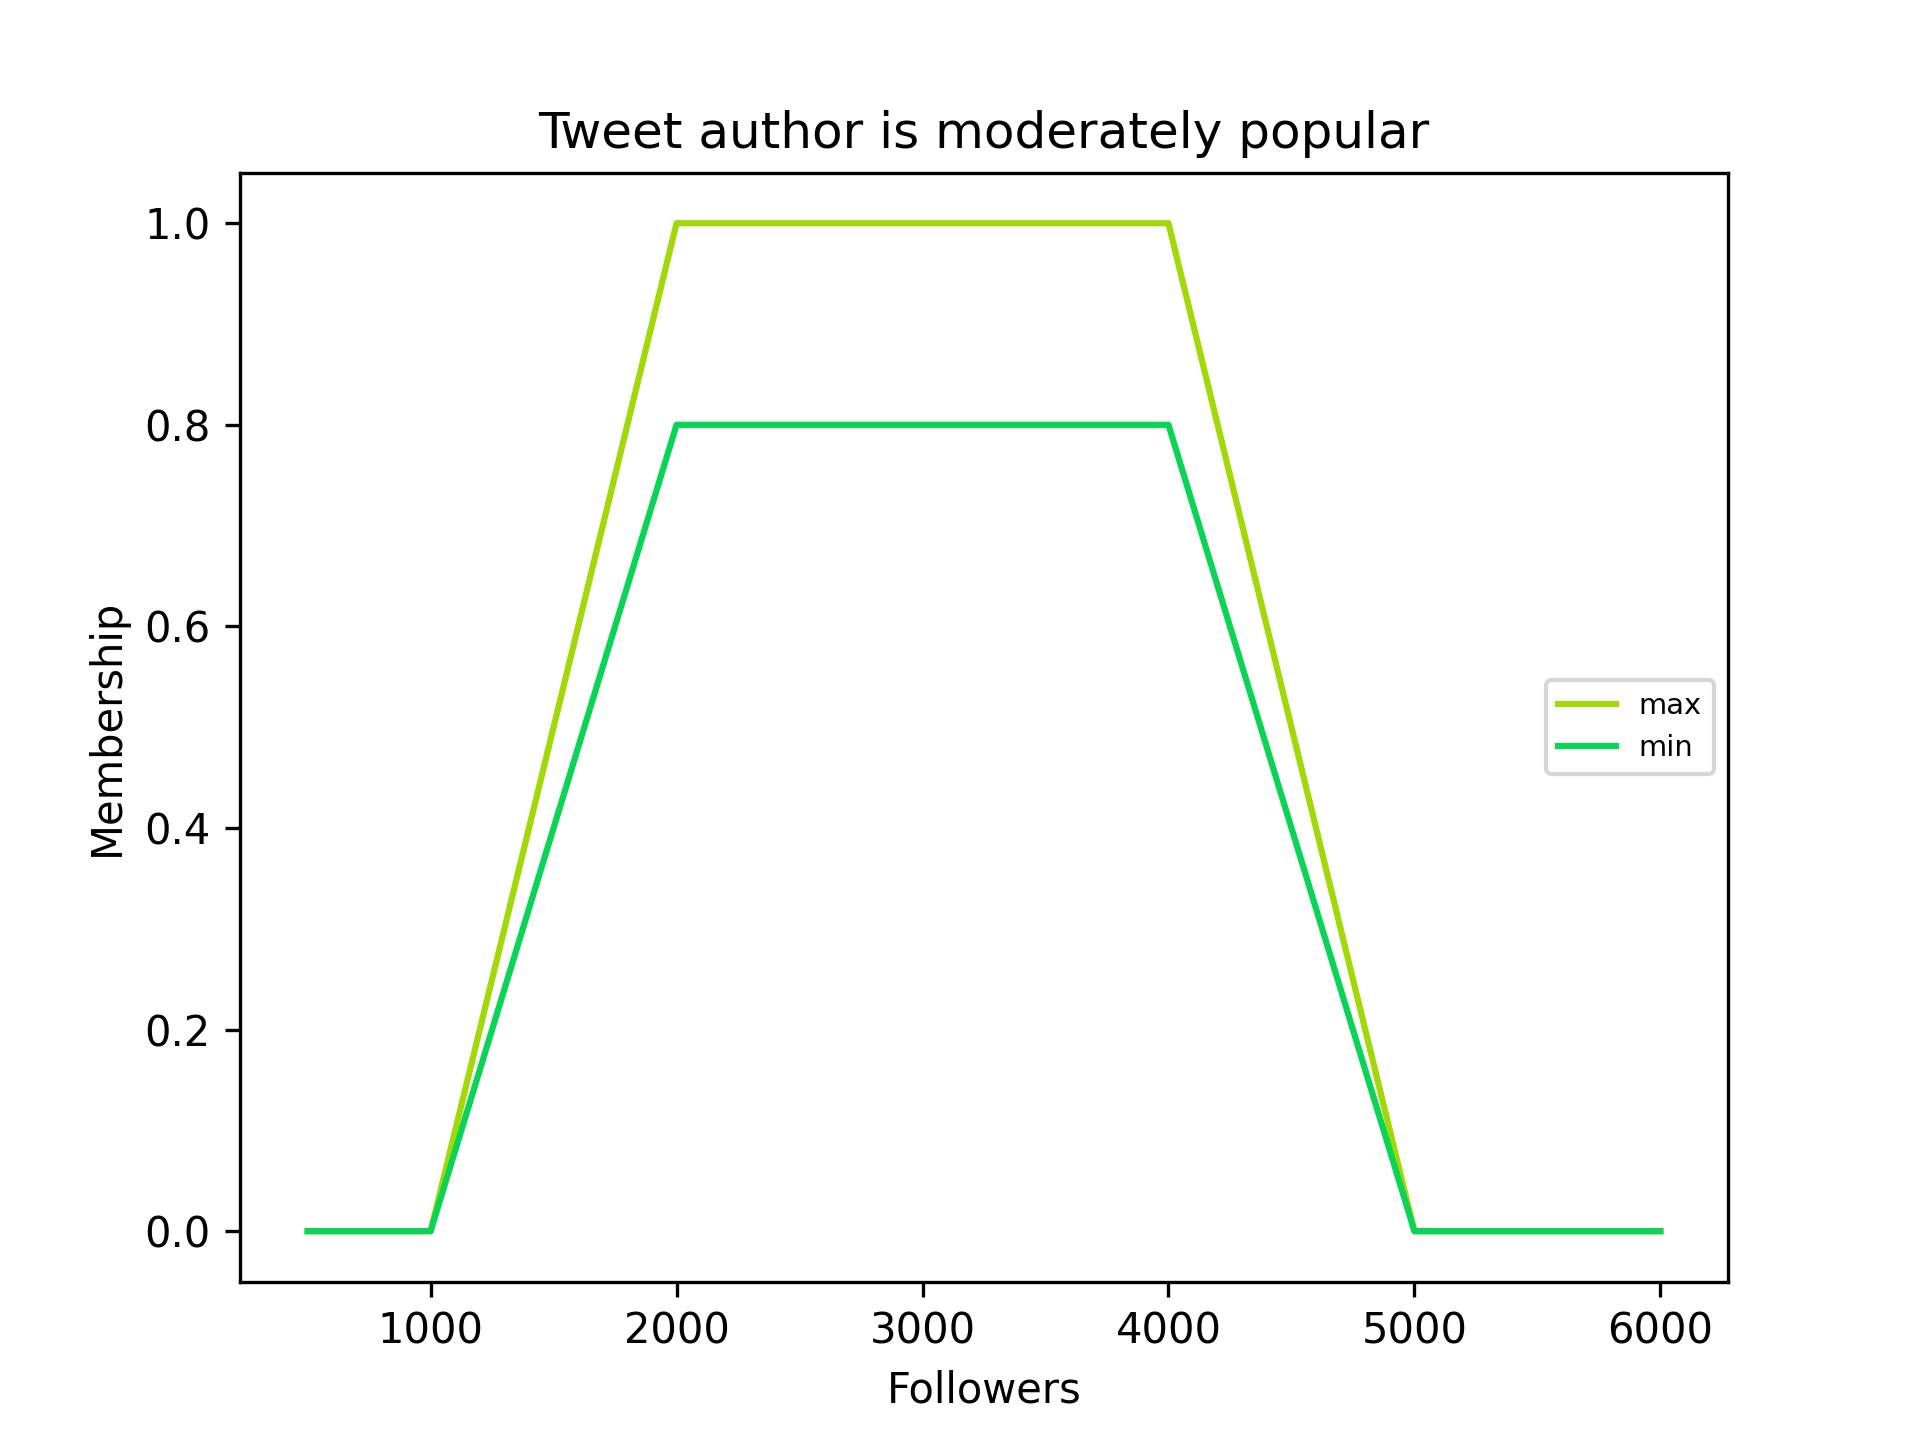
\includegraphics[width=1\textwidth]{resources/stage3/Tweet author is moderately popular.png}
    \caption{Przedziałowa funkcja przynależności dla atrybutu followers}
    \label{moderately_popular}
\end{figure}

\begin{figure}[H]
    \centering
    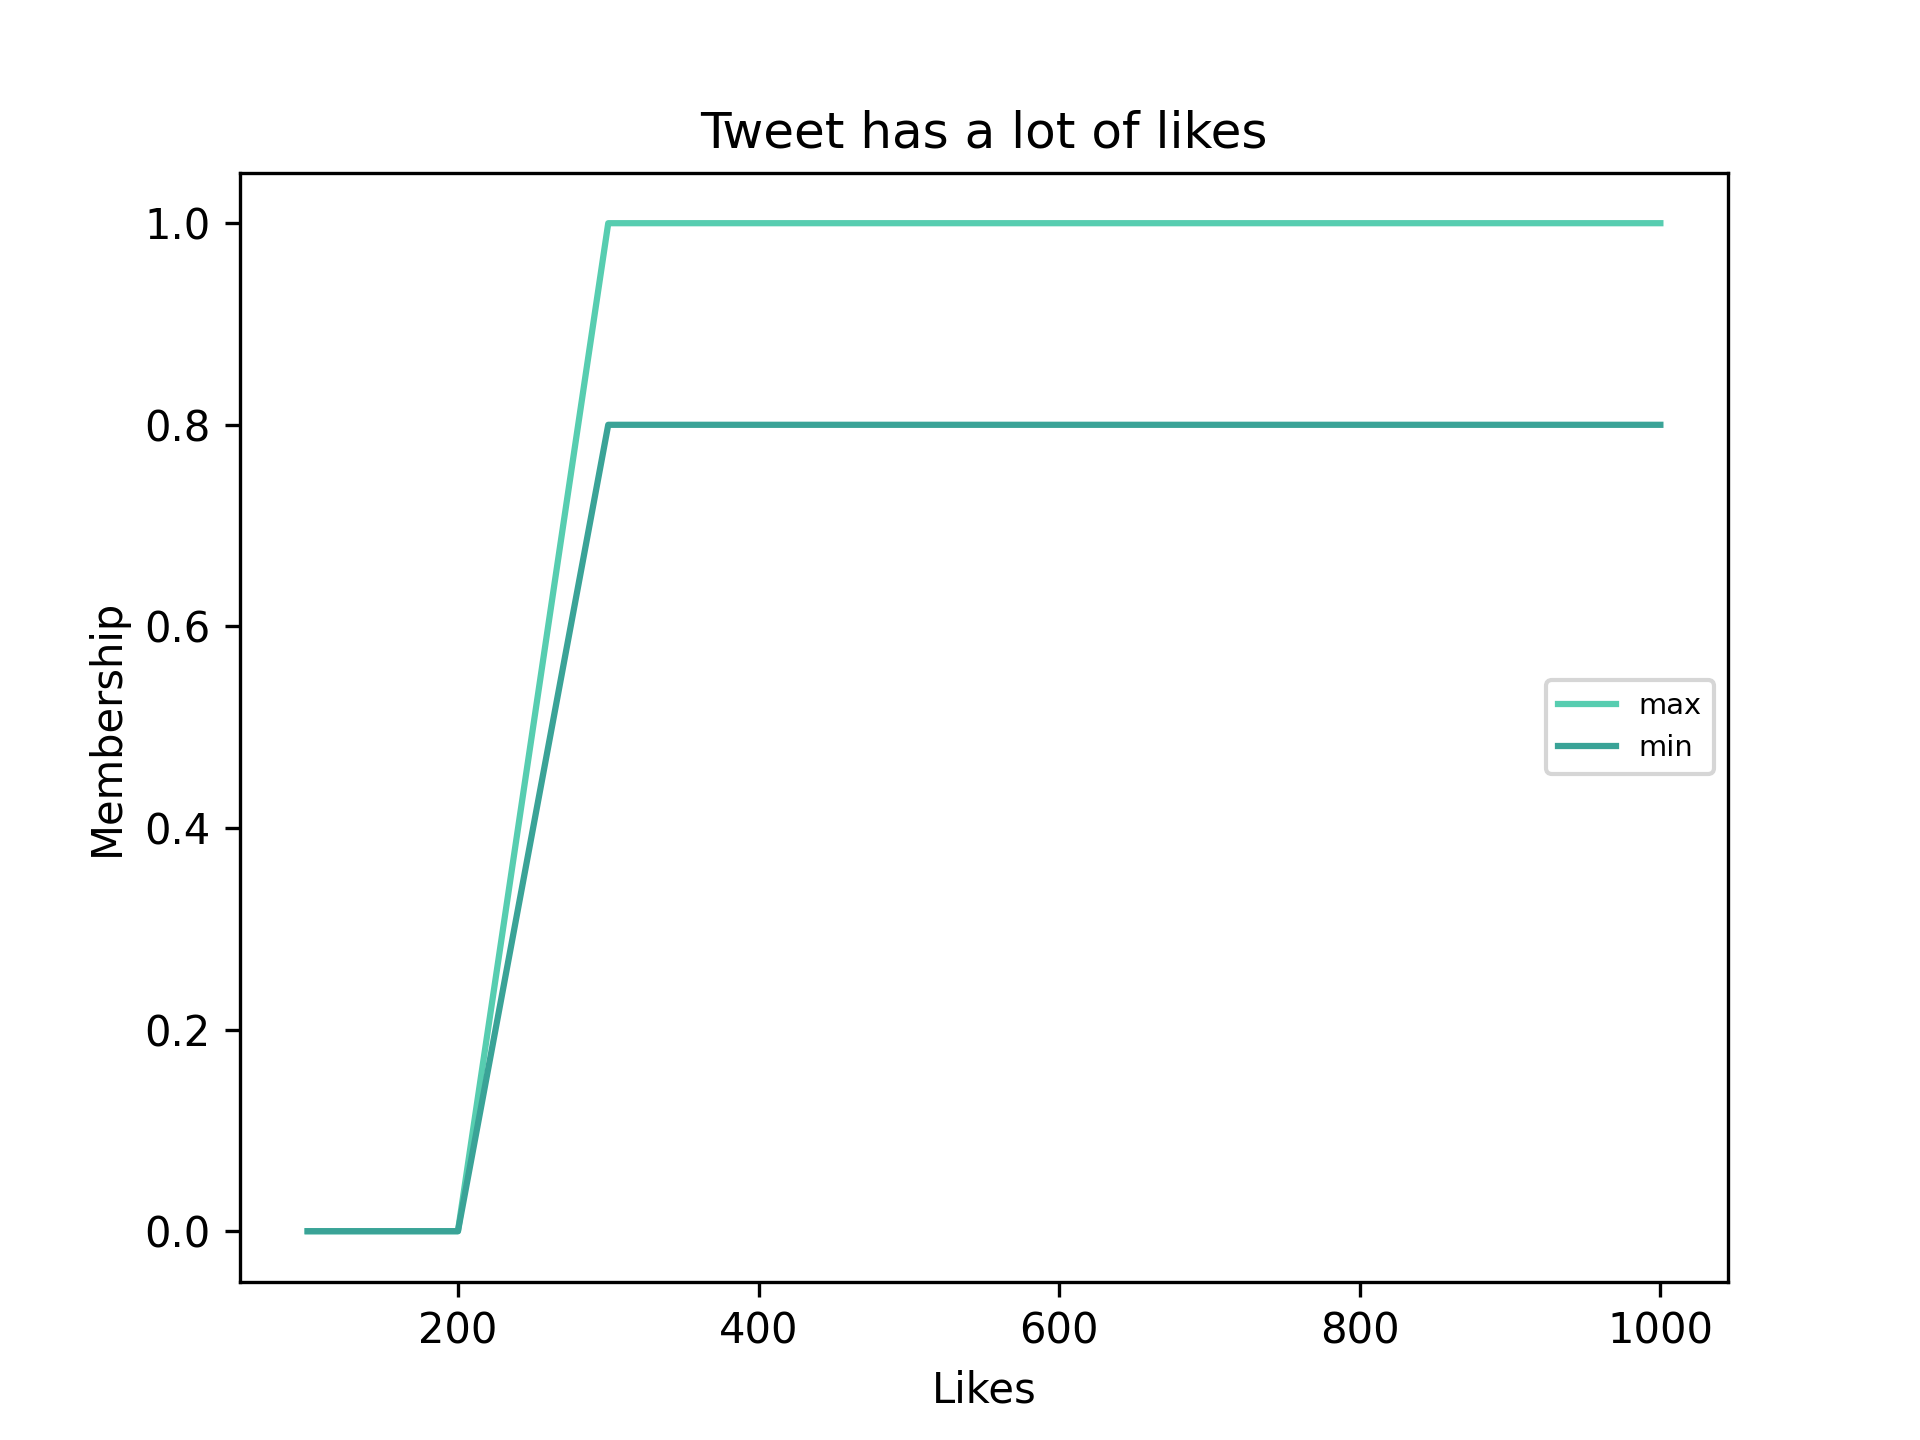
\includegraphics[width=1\textwidth]{resources/stage3/Tweet has a lot of likes.png}
    \caption{Przedziałowa funkcja przynależności dla atrybutu likes}
    \label{very_liked}
\end{figure}

\begin{figure}[H]
    \centering
    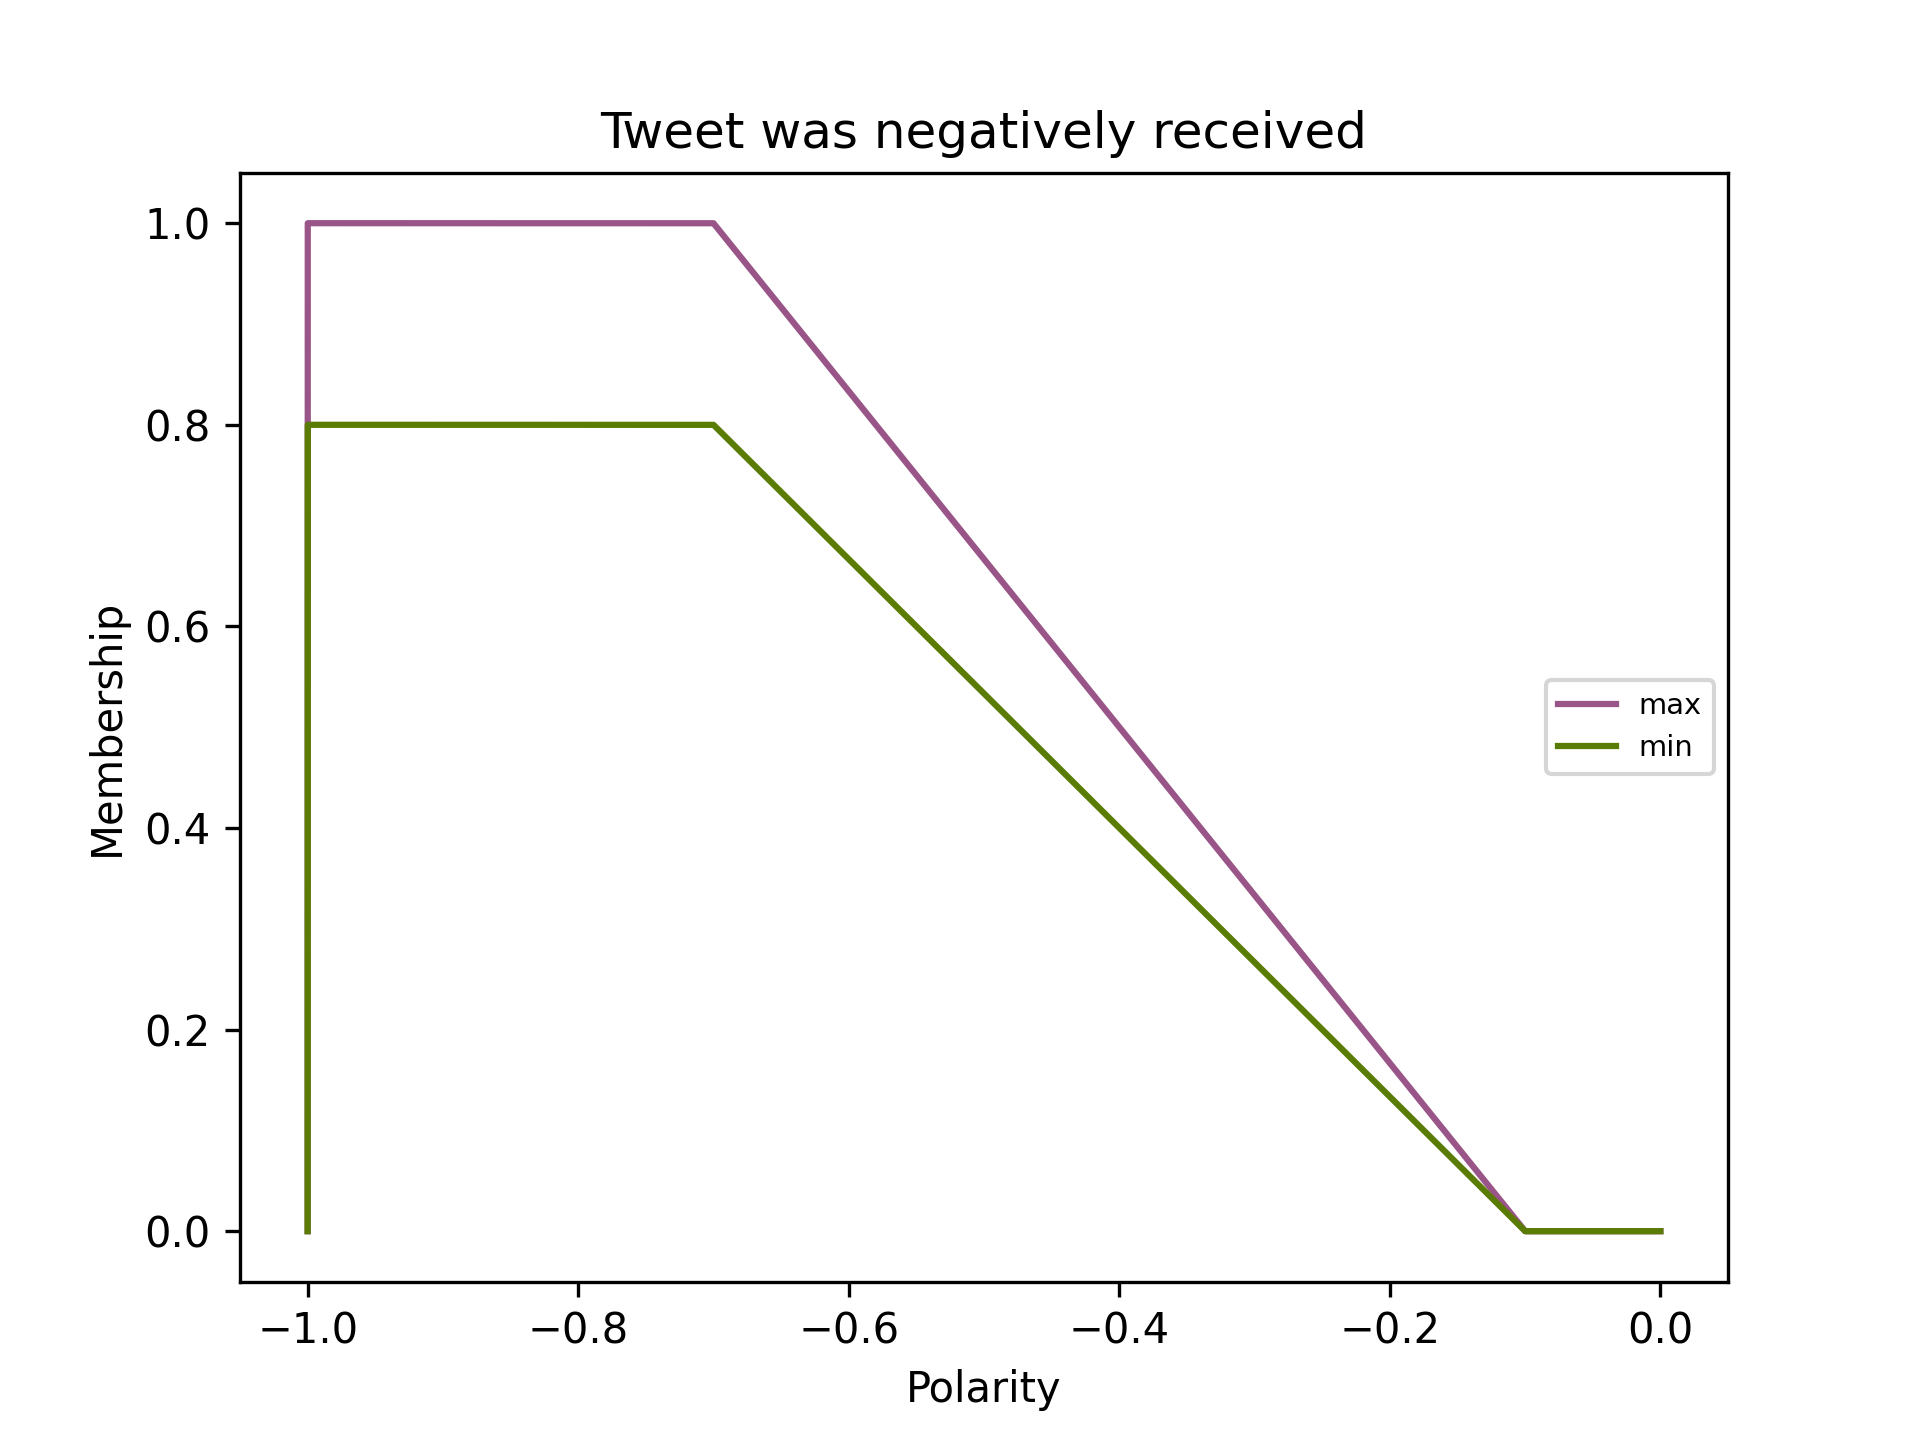
\includegraphics[width=1\textwidth]{resources/stage3/Tweet was negatively received.png}
    \caption{Przedziałowa funkcja przynależności dla atrybutu polarity}
    \label{negatively_received}
\end{figure}

Ponownie dla każdego tweeta wyliczono wartości przedziałowych funkcji przynależności i zapisano w arkuszu \textit{Fuzzy interval membership}. Poglądowa część zaprezentowana jest w Tabeli \ref{fuzzy_interval}

\begin{landscape}
\mbox{}\vfill
\begin{table}[H]
    \caption{Wartości przedziałowych funkcji przynależności tweetów}
    \label{fuzzy_interval}
    \centering
    \resizebox{1.85\textwidth}{!}{
    \begin{tabular}{llllllll}
        \hline
        \multicolumn{1}{|l|}{Author} &
          \multicolumn{1}{l|}{Tweet} &
          \multicolumn{1}{l|}{\begin{tabular}[c]{@{}l@{}}Tweet has a lot of \\ likes (min)\end{tabular}} &
          \multicolumn{1}{l|}{\begin{tabular}[c]{@{}l@{}}Tweet has a lot of \\ likes (max)\end{tabular}} &
          \multicolumn{1}{l|}{\begin{tabular}[c]{@{}l@{}}Tweet was negatively\\ received (min)\end{tabular}} &
          \multicolumn{1}{l|}{\begin{tabular}[c]{@{}l@{}}Tweet was negatively\\ received (max)\end{tabular}} &
          \multicolumn{1}{l|}{\begin{tabular}[c]{@{}l@{}}Tweet author is moderately\\ popular (min)\end{tabular}} &
          \multicolumn{1}{l|}{\begin{tabular}[c]{@{}l@{}}Tweet author is moderately\\ popular (max)\end{tabular}} \\ \hline
        \multicolumn{1}{|l|}{ECOWARRIORSS} &
          \multicolumn{1}{l|}{\{Treść\}} &
          \multicolumn{1}{l|}{0} &
          \multicolumn{1}{l|}{0} &
          \multicolumn{1}{l|}{0} &
          \multicolumn{1}{l|}{0} &
          \multicolumn{1}{l|}{0} &
          \multicolumn{1}{l|}{0} \\ \hline
        \multicolumn{1}{|l|}{ElsevierEnergy} &
          \multicolumn{1}{l|}{\{Treść\}} &
          \multicolumn{1}{l|}{0} &
          \multicolumn{1}{l|}{0} &
          \multicolumn{1}{l|}{0} &
          \multicolumn{1}{l|}{0} &
          \multicolumn{1}{l|}{0} &
          \multicolumn{1}{l|}{0} \\ \hline
        \multicolumn{1}{|l|}{siwarr5} &
          \multicolumn{1}{l|}{\{Treść\}} &
          \multicolumn{1}{l|}{0} &
          \multicolumn{1}{l|}{0} &
          \multicolumn{1}{l|}{0} &
          \multicolumn{1}{l|}{0} &
          \multicolumn{1}{l|}{0} &
          \multicolumn{1}{l|}{0} \\ \hline
        \multicolumn{1}{|l|}{EDITORatWORK} &
          \multicolumn{1}{l|}{\{Treść\}} &
          \multicolumn{1}{l|}{0} &
          \multicolumn{1}{l|}{0} &
          \multicolumn{1}{l|}{0} &
          \multicolumn{1}{l|}{0} &
          \multicolumn{1}{l|}{0,65} &
          \multicolumn{1}{l|}{0,81} \\ \hline
        \multicolumn{1}{|l|}{EDITORatWORK} &
          \multicolumn{1}{l|}{\{Treść\}} &
          \multicolumn{1}{l|}{0} &
          \multicolumn{1}{l|}{0} &
          \multicolumn{1}{l|}{0} &
          \multicolumn{1}{l|}{0} &
          \multicolumn{1}{l|}{0,65} &
          \multicolumn{1}{l|}{0,81} \\ \hline
        \multicolumn{1}{|l|}{mapsofworld} &
          \multicolumn{1}{l|}{\{Treść\}} &
          \multicolumn{1}{l|}{0} &
          \multicolumn{1}{l|}{0} &
          \multicolumn{1}{l|}{0,03} &
          \multicolumn{1}{l|}{0,04} &
          \multicolumn{1}{l|}{0} &
          \multicolumn{1}{l|}{0} \\ \hline
        \multicolumn{1}{|l|}{EnvirHealthNews} &
          \multicolumn{1}{l|}{\{Treść\}} &
          \multicolumn{1}{l|}{0} &
          \multicolumn{1}{l|}{0} &
          \multicolumn{1}{l|}{0} &
          \multicolumn{1}{l|}{0} &
          \multicolumn{1}{l|}{0} &
          \multicolumn{1}{l|}{0} \\ \hline
         &
           &
           &
           &
          ... &
           &
           &
           \\ \hline
        \multicolumn{1}{|l|}{TheDailyClimate} &
          \multicolumn{1}{l|}{\{Treść\}} &
          \multicolumn{1}{l|}{0} &
          \multicolumn{1}{l|}{0} &
          \multicolumn{1}{l|}{0} &
          \multicolumn{1}{l|}{0} &
          \multicolumn{1}{l|}{0} &
          \multicolumn{1}{l|}{0} \\ \hline
    \end{tabular}   }
\end{table}
\vfill\mbox{}
\end{landscape}

\subsection{Wyliczenie współczynnika R}

Do wyliczenia współczynnika R wybrano atrybuty polarity i followers. Każdemu z nich nadano 5 etykiet i stworzono funkcje przynależności:

\begin{itemize}
    \item Dla atrybutu polarity nadano etykiety:
    \begin{itemize}
        \item Negatively received
        \item Moderately negatively received
        \item Neutrally received
        \item Moderately positively received
        \item Positively receive
    \end{itemize}
    których funkcje przynależności pokazano na Rysunku \ref{receival}
    \item Dla atrybutu followers nadano etykiety:
    \begin{itemize}
        \item Not popular
        \item Little popular
        \item Moderately popular
        \item Very popular
        \item Extremely popular
    \end{itemize}
    których funkcje przynależności pokazano na Rysunku \ref{popularity}
\end{itemize}

\begin{figure}[H]
    \centering
    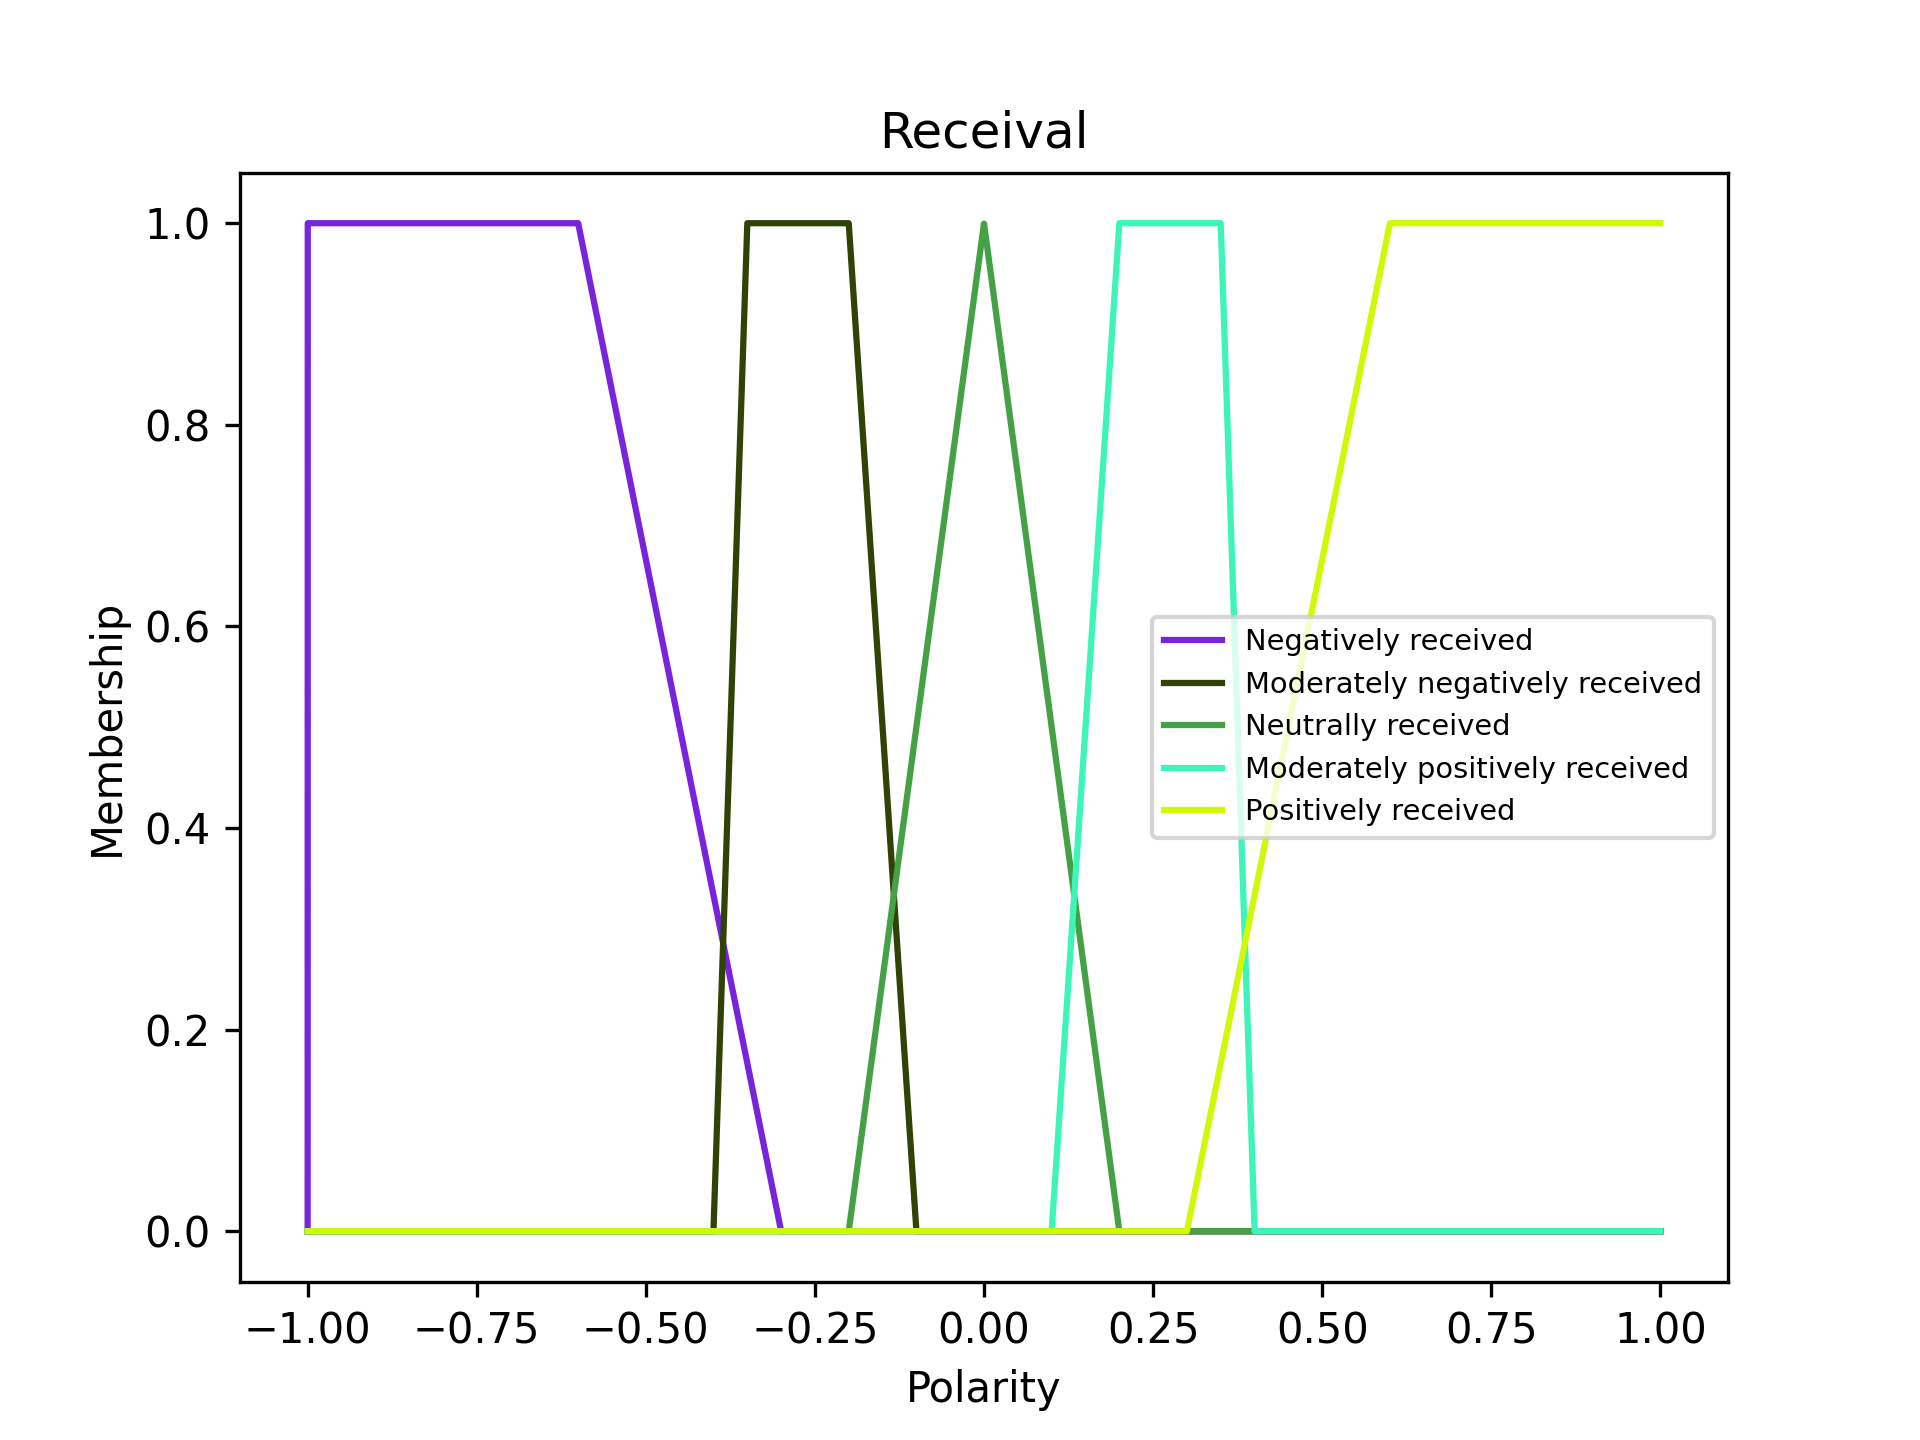
\includegraphics[width=1\textwidth]{resources/stage3/Receival.png}
    \caption{Funkcje przynależności dla atrybutu polarity}
    \label{receival}
\end{figure}

\begin{figure}[H]
    \centering
    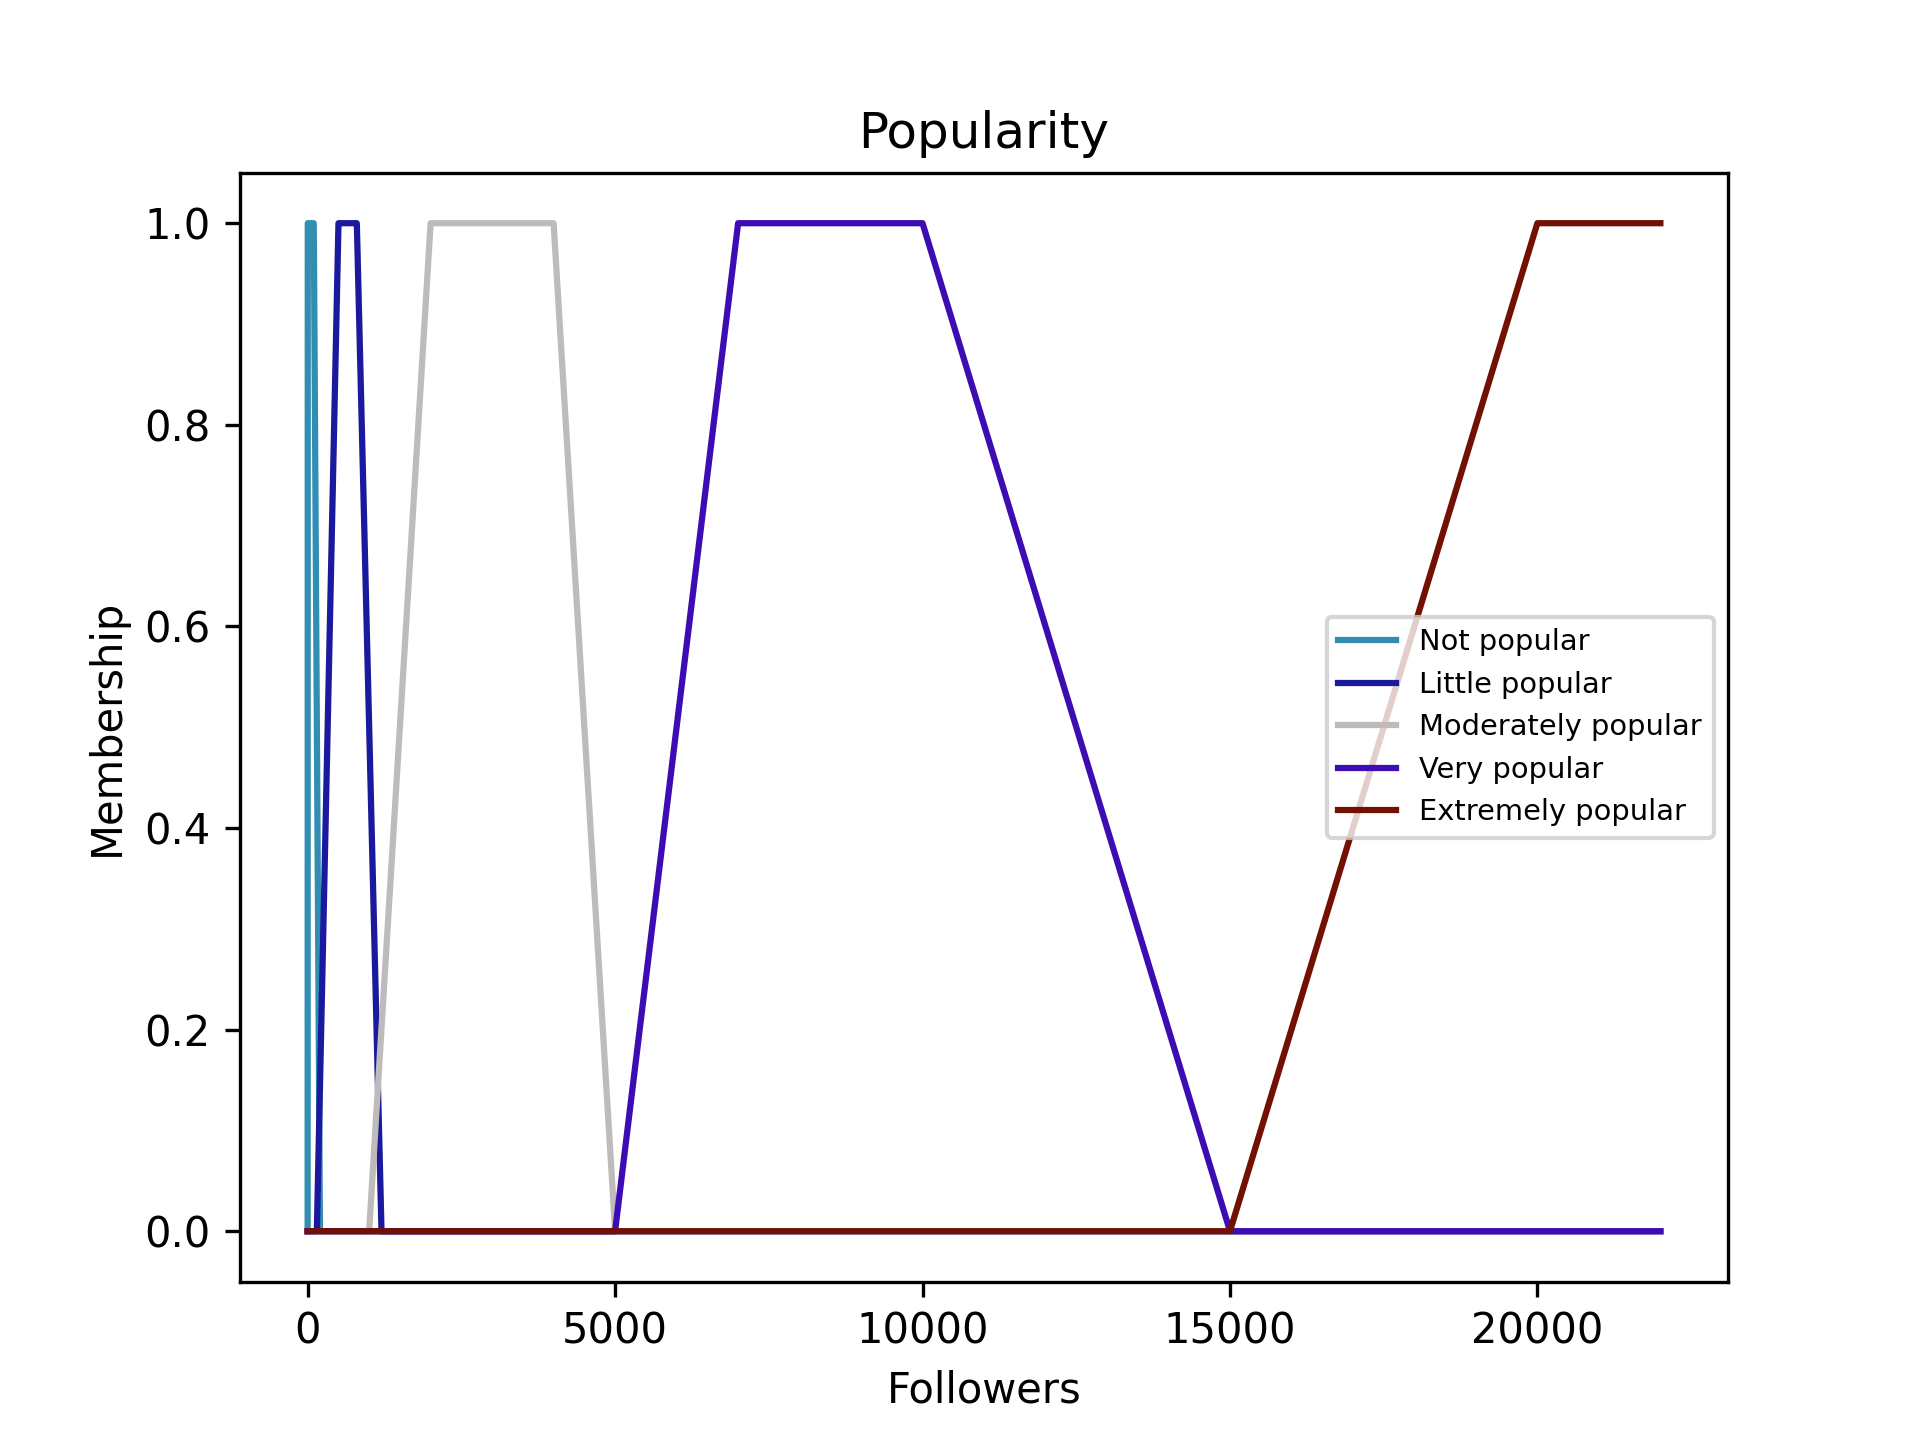
\includegraphics[width=1\textwidth]{resources/stage3/Popularity.png}
    \caption{Funkcje przynależności dla atrybutu followers}
    \label{popularity}
\end{figure}

Dla każdego tweeta wyliczono współczynnik R i zapisano w arkuszu \textit{Receival to popularity R coef}. Część wyników pokazuje Tabela \ref{r}

\begin{table}[H]
    \caption{Wartości przedziałowych funkcji przynależności tweetów}
    \label{r}
    \centering
    \begin{tabular}{lll}
        \hline
        \multicolumn{1}{|l|}{Author} & \multicolumn{1}{l|}{Tweet} & \multicolumn{1}{l|}{\begin{tabular}[c]{@{}l@{}}Receival to popularity\\ R coefficient\end{tabular}} \\ \hline
        \multicolumn{1}{|l|}{ECOWARRIORSS}    & \multicolumn{1}{l|}{\{Treść\}} & \multicolumn{1}{l|}{0}        \\ \hline
        \multicolumn{1}{|l|}{ElsevierEnergy}  & \multicolumn{1}{l|}{\{Treść\}} & \multicolumn{1}{l|}{0,37} \\ \hline
        \multicolumn{1}{|l|}{siwarr5}         & \multicolumn{1}{l|}{\{Treść\}} & \multicolumn{1}{l|}{0}        \\ \hline
        \multicolumn{1}{|l|}{EDITORatWORK}    & \multicolumn{1}{l|}{\{Treść\}} & \multicolumn{1}{l|}{0,81}    \\ \hline
        \multicolumn{1}{|l|}{EDITORatWORK}    & \multicolumn{1}{l|}{\{Treść\}} & \multicolumn{1}{l|}{0,81}    \\ \hline
        \multicolumn{1}{|l|}{mapsofworld}     & \multicolumn{1}{l|}{\{Treść\}} & \multicolumn{1}{l|}{0}        \\ \hline
        \multicolumn{1}{|l|}{EnvirHealthNews} & \multicolumn{1}{l|}{\{Treść\}} & \multicolumn{1}{l|}{0,95}   \\ \hline
                                              & \multicolumn{1}{c}{...}        &                               \\ \hline
        \multicolumn{1}{|l|}{TheDailyClimate} & \multicolumn{1}{l|}{\{Treść\}} & \multicolumn{1}{l|}{0}        \\ \hline
    \end{tabular}
\end{table}

\section{Wnioski}

\begin{enumerate}
    \item Wykorzystana metoda porównywania tekstu nie jest symetryczna
    \item Do skonstruowania odpowiedniej etykiety i funkcji przynależności wymagana jest wiedza ekspercka 
\end{enumerate}

\newpage
\nocite{*}
\begin{thebibliography}{}

    \bibitem{db}
    \textsl{Zbiór danych z wpisami z portalu Tweeter, }
    \url{ https://www.kaggle.com/joseguzman/climate-sentiment-in-twitter?select=Climate_twitter.csv}
    \text{ [dostęp: 15.11.2020]}
    
\end{thebibliography}

\end{document}
